% !TEX root = tracking.tex
\section{Introduction}
 Currently there is a great interest both in research and industry to find methods of path planning and model-predictive control (MPC) for autonomous quadrotors and other vehicles.  These vehicles must be able to plan and execute a path in real-time without violating safety constraints. This is a very difficult challenge: the need for fast planning is generally at odds with the need for maintaining safety. In order to achieve real-time planning and model-predictive control (MPC) for any environment with static obstacles researchers typically must use highly simplified model dynamics. This results in a tracking error between the planned path and the true high-dimensional system. This concept is illustrated in Figure \ref{fig:chasing}, where the path was planned using vehicle 1, but the real vehicle 2 cannot follow this path exactly. In addition, most current planners do not consider the effect of external disturbance (e.g. wind) on the resulting tracking error. This tracking error due to the simplified dynamics and lack of disturbances can lead to unsafe situations in which the planned path may be safe, but the actual vehicle trajectory crashes into an obstacle or other unsafe region.

We propose precomputing a bound on the possible tracking error between the path planned by the simplified model and the true high-dimensional vehicle dynamics. We compute this by using Hamilton Jacobi reachability analysis to analyze a capture-avoid game in relative coordinates between the true high-dimensional vehicle dynamics and a 'virtual' vehicle that uses the simplified model dynamics. Additional disturbances can be included in this analysis. The result is an invariant set of relative states around the virtual simplified vehicle that provides bounds on the possible tracking error between the two systems. This precomputed set also provides a look-up table to determine the optimal control required for the true vehicle to remain as close as possible to the virtual simplified vehicle. This set captures all deviations due to nonlinearities and disturbance in the true system.

\begin{figure}
	\centering
	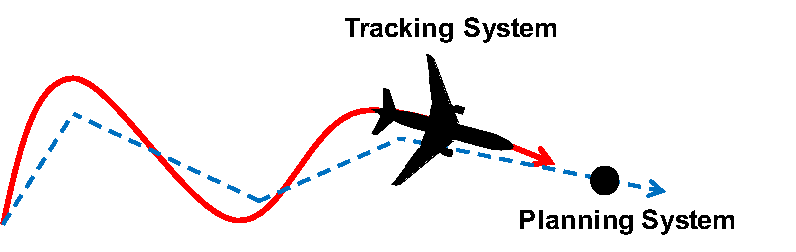
\includegraphics[width=0.47\textwidth]{fig/chasing}
	\caption{filler image about planes chasing each other}
	\label{fig:chasing}
\end{figure}

We can couple this precomputed set with any model-preditive control method (MPC) that uses the simplified dynamics. As the MPC plans with the virtual vehicle, the true vehicle will use the relative state between itself and the virtual vehicle to look up the optimal control that will reduce tracking error. We can guarantee safety with the MPC method by expanding all encountered obstacles by the precomputed tracking error bound. The only additional computation required in real-time will be to access a look-up table with the optimal control for a given state.

We show our results in blablabla